Relaciona la imagen con  el tipo de onda electromagnética que está involucrada.
\begin{multicols}{2}

    \begin{choices}
        \choice Rayos X                 \vspace{2cm}
        \choice Rayos gamma             \vspace{2cm}
        \choice Radiación infraroja     \vspace{2cm}
        \choice Rayos ultravioleta      \vspace{2cm}
    \end{choices}
    
    \columnbreak

    \begin{parts}
        \part \fillin[D][1cm] \adjustbox{valign=t}{
\includegraphics[width=0.2\textwidth ]{../images/SINFI_U3_AC77_IMG4.png} }
        \part \fillin[C][1cm] \adjustbox{valign=t}{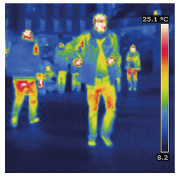
\includegraphics[width=0.2\textwidth ]{../images/SINFI_U3_AC77_IMG5.png} }
        \part \fillin[B][1cm] \adjustbox{valign=t}{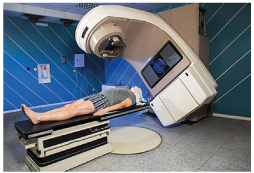
\includegraphics[width=0.2\textwidth ]{../images/SINFI_U3_AC77_IMG6.png} }
        \part \fillin[A][1cm] \adjustbox{valign=t}{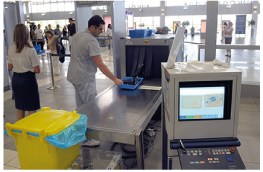
\includegraphics[width=0.2\textwidth ]{../images/SINFI_U3_AC77_IMG7.png} }
    \end{parts}
\end{multicols}